% Sourdough starter schedule: weekly fridge routine and back-to-back bakes.
% Compile: latexmk -pdf starter_schedule.tex   (from docs/)
% Edit the amounts in the "Recipe numbers" block; the tables pick them up.
\documentclass[11pt]{article}
\usepackage[letterpaper,margin=0.8in]{geometry}
\usepackage[T1]{fontenc}
\usepackage{lmodern}
\usepackage{microtype}
\usepackage{booktabs}
\usepackage{tabularx}
\usepackage{enumitem}
\usepackage{amsmath,amssymb}
\usepackage{xcolor}
\usepackage{tikz}
\usetikzlibrary{arrows.meta,positioning}
\usepackage[hidelinks]{hyperref}

\setlist{itemsep=2pt,topsep=4pt}
\newcommand{\todo}{\item[$\square$]}
\newcommand{\feed}[3]{#1\,:\,#2\,:\,#3}   % starter : flour : water

% ---- Recipe numbers (grams) --------------------------------------------
% Mother kept in the fridge
\newcommand{\motherG}{35}
% Levain build for the Perfect Loaf no-knead (needs 153 g)
\newcommand{\plNeed}{153}
\newcommand{\plS}{30}\newcommand{\plF}{75}\newcommand{\plW}{75}
\newcommand{\plTotal}{180}
% Levain build for the second recipe (needs 120 g)
\newcommand{\rbNeed}{120}
\newcommand{\rbS}{25}\newcommand{\rbF}{60}\newcommand{\rbW}{60}
\newcommand{\rbTotal}{145}
% After-bake refresh of the leftover
\newcommand{\refF}{10}\newcommand{\refW}{10}
% Weekly maintenance (no bake)
\newcommand{\mainS}{10}\newcommand{\mainF}{12}\newcommand{\mainW}{12}
% Times
\newcommand{\buildTime}{9\,PM}
\newcommand{\readyTime}{9--10\,AM}
% -------------------------------------------------------------------------

\title{Sourdough Starter Schedule}
\author{Kris Ezra}
\date{Revised \today}

\begin{document}
\maketitle
\vspace{-1em}

\section*{Overview}

One Weck jar holds about \motherG\,g of whole wheat starter at 100\% hydration, and
it lives in the fridge. The night before a bake, the whole mother is fed up into the
levain. Whatever is left after you take the levain becomes the next mother, so a bake
week produces almost no discard.

\begin{itemize}
  \item \textbf{Baking:} decide by about \buildTime{} the night before. Feed the jar,
        leave it on the counter overnight, take the levain in the morning.
  \item \textbf{Not baking:} feed it once a week and put it straight back in the
        fridge. About 25\,g of discard per week.
  \item \textbf{Baking several days in a row:} repeat the night-before build each
        evening. Between bakes the jar waits in the fridge.
  \item \textbf{A day or two late:} no harm; feed on the day you remember. This routine
        has no twice-daily feeds left to miss.
  \item \textbf{Vacation:} plan for it (see Vacation). After two weeks in the fridge the
        starter took about four feeds to recover (Oct~30 to Nov~2, 2026).
\end{itemize}

Times assume a pantry around 68\,\textdegree F. Weights are grams; \feed{30}{75}{75}
means starter\,:\,flour\,:\,water.

\begin{center}
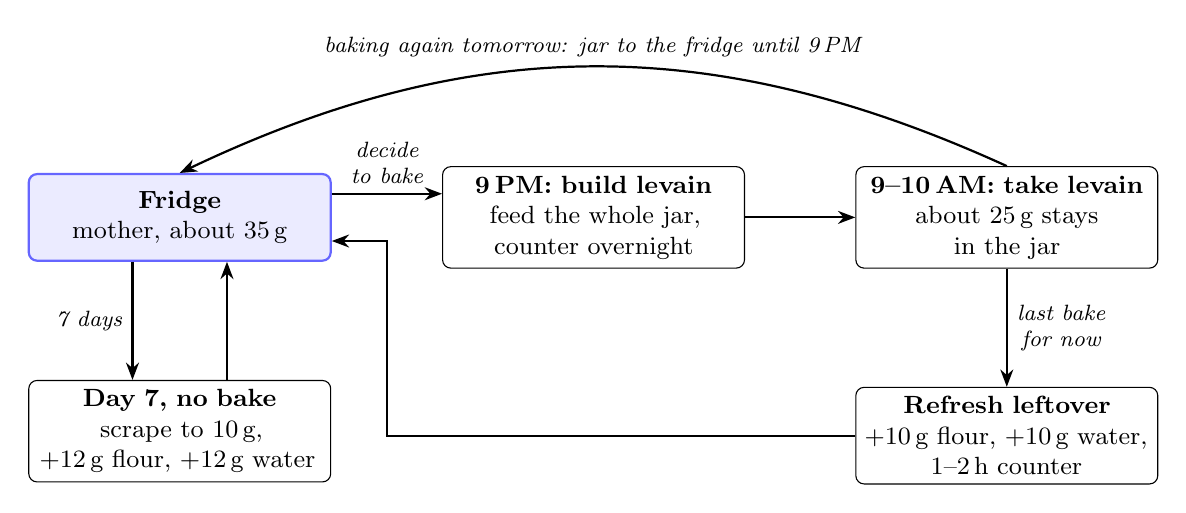
\begin{tikzpicture}[
  font=\small,
  box/.style={draw, rounded corners=3pt, align=center, minimum height=1.1cm, text width=3.6cm},
  main/.style={box, fill=blue!8, draw=blue!60, thick},
  arr/.style={-{Stealth[length=2.2mm]}, thick},
  lab/.style={font=\footnotesize\itshape, align=center}
]
  \node[main] (fridge) {\textbf{Fridge}\\mother, about \motherG\,g};
  \node[box, right=1.4cm of fridge] (build) {\textbf{\buildTime: build levain}\\feed the whole jar,\\counter overnight};
  \node[box, right=1.4cm of build] (take) {\textbf{\readyTime: take levain}\\about 25\,g stays\\in the jar};
  \node[box, below=1.5cm of take] (refresh) {\textbf{Refresh leftover}\\+\refF\,g flour, +\refW\,g water,\\1--2\,h counter};
  \node[box, below=1.5cm of fridge] (weekly) {\textbf{Day 7, no bake}\\scrape to \mainS\,g,\\+\mainF\,g flour, +\mainW\,g water};

  \draw[arr] ([yshift=3mm]fridge.east) -- node[lab, above] {decide\\to bake} ([yshift=3mm]build.west);
  \draw[arr] (build) -- (take);
  \draw[arr] (take) -- node[lab, right] {last bake\\for now} (refresh);
  \draw[arr] (take.north) to[bend right=25] node[lab, above] {baking again tomorrow: jar to the fridge until \buildTime} (fridge.north);
  \draw[arr] (refresh.west) -| ([xshift=7mm,yshift=-3mm]fridge.east) -- ([yshift=-3mm]fridge.east);
  \draw[arr] ([xshift=-6mm]fridge.south) -- node[lab, left] {7 days} ([xshift=-6mm]weekly.north);
  \draw[arr] ([xshift=6mm]weekly.north) -- ([xshift=6mm]fridge.south);
\end{tikzpicture}
\end{center}

\section*{Weekly fridge routine}

\subsection*{Bake week}

\begin{enumerate}
  \item \textbf{Night before, about \buildTime.} Take the jar out. Scrape it down to
        the starter amount below (by gross weight, see Tools), then add flour and
        water and stir in the walls. Use water around 80\,\textdegree F to offset the
        cold start. Mark the level with a rubber band.
  \item \textbf{Morning, about \readyTime.} It is ready when it has roughly
        doubled (past rises were 1.5--1.9$\times$), the top is domed, and it is still
        rising or just flat. Take the levain.
  \item \textbf{After taking the levain.} If you bake again tomorrow, put the jar
        straight in the fridge. Otherwise refresh the leftover: add \refF\,g flour and
        \refW\,g water, leave it 1--2\,h on the counter, then fridge.
\end{enumerate}

\begin{center}
\begin{tabular}{@{}lccc@{}}
\toprule
Recipe & Levain needed & Build (s\,:\,f\,:\,w) & Total \\
\midrule
Perfect Loaf no-knead & \plNeed\,g & \feed{\plS}{\plF}{\plW} & \plTotal\,g \\
Second recipe          & \rbNeed\,g & \feed{\rbS}{\rbF}{\rbW} & \rbTotal\,g \\
\bottomrule
\end{tabular}
\end{center}

Each build leaves about 25\,g in the jar after the levain is taken, allowing a few
grams lost on the walls and spatula.

\subsection*{No-bake week}

On day~7 with no bake planned: take the jar out, scrape it down to \mainS\,g, add
\mainF\,g flour and \mainW\,g water, leave it 1--2\,h on the counter, then fridge.
That leaves about 34\,g, enough for the next build.

\subsection*{If the first build is slow}

Building straight from a week-old fridge starter has not been tested yet. If the
levain is not ready by mid-morning, add a wake-up feed next time: around noon on the
day before, take 10\,g into a clean jar with 20\,g flour and 20\,g water, leave it on
the counter, and use 30\,g of it for the \buildTime{} build.

\section*{Vacation}

Before leaving, give the weekly maintenance feed and refrigerate it right away, with
no counter time. On return, expect three or four feeds over two days before a
night-before build behaves normally: 10\,g starter with 20\,g flour and 20\,g water,
morning and evening, until it doubles in about 8--10\,h. The dried backup covers a
total loss.

\section*{Baking several days in a row}

Repeat the night-before build each evening, using whatever the morning left in the
jar (about 25\,g) with the same flour and water. Keep the jar in the fridge between
the morning and the evening build, so the starter does not sit warm past its peak
for 12\,h.

\begin{center}
\begin{tabularx}{\linewidth}{@{}lX@{}}
\toprule
When & What \\
\midrule
Day 0, \buildTime & Build from the fridge mother (table above). \\
Day 1, morning   & Take the levain, bake. Jar to the fridge. \\
Day 1, \buildTime & Build again on the leftover, same flour and water. \\
Day 2, morning   & Take the levain, bake. Jar to the fridge. \\
Day 2, \buildTime & Build again (third bake), or refresh with \refF\,:\,\refW{} and stop. \\
Day 3, morning   & Last bake: refresh the leftover, 1--2\,h counter, fridge. Back to the weekly routine. \\
\bottomrule
\end{tabularx}
\end{center}

\section*{Quick reference: ready time vs.\ starter amount}

Run~1 (whole wheat, 100\% hydration, about 68--69\,\textdegree F) fit
\[
  t_{90} \approx 4.4 + 3.8\,\ln\!\left(\frac{\text{total}}{\text{starter}}\right)\ \text{hours},
\]
where $t_{90}$ is the time to 90\% of the rise. Halving the starter adds about 2.6\,h.
For a \plTotal\,g build:

\begin{center}
\begin{tabular}{@{}lcccccc@{}}
\toprule
Starter (g)        & 15 & 20 & 25 & 30 & 40 & 60 \\
Ready after (h)    & 13.8 & 12.8 & 11.9 & 11.2 & 10.1 & 8.6 \\
\bottomrule
\end{tabular}
\end{center}

\begin{itemize}
  \item Treat these as $\pm 2$\,h. The same feed on different days varied by
        1.5--3\,h, most likely from temperature, which was never recorded.
  \item The formula was measured with room-temperature starter. A fridge-cold start
        probably adds an hour or two; not yet measured.
  \item Warmer is faster, cooler is slower. To shift the ready time, change the
        starter amount using the table.
  \item It holds near the peak for several hours at these amounts (13\,h+ in one
        Run~1 jar), so a late morning is usually fine.
\end{itemize}

\section*{Tools and measuring}

\begin{itemize}
  \item \textbf{Scale.} At least 2\,kg capacity (bread doughs); 3--5\,kg is easier.
        1\,g resolution is enough for routine feeds. The current scale swallows slow
        additions even away from zero, so: add each ingredient in one quick dump,
        and confirm by lifting the jar and setting it back down. When buying, look
        for zero tracking that can be switched off, and test it with a known weight:
        a US nickel is 5.0\,g, a penny 2.5\,g. Slide one onto a loaded scale slowly;
        the reading should rise by that amount.
  \item \textbf{Starter by gross weight.} Write each jar's empty weight on it (or etch
        it). Target = jar + starter, e.g.\ jar + \plS\,g. Scrape out until the scale
        reads the target; the residue on the walls counts toward the starter.
  \item \textbf{Water by volume.} 1\,mL of water = 1\,g, so no scale is needed.
        A 60\,mL catheter-tip syringe covers 10--60\,g in one pull and the small
        refreshes exactly. A 100\,mL graduated cylinder takes the 60--75\,g build
        water in one fill.
  \item \textbf{Flour by pre-portioning.} Weigh build and maintenance portions into
        lidded cups in one sitting (75\,g, 60\,g, 12\,g), so each feed is one dump.
        Hold off on measuring scoops until the hydration is settled.
\end{itemize}

\section*{Open questions and tests}

\begin{itemize}[label={}]
  \todo \textbf{Fridge-to-levain dry run.} Next bake: build straight from the fridge
        mother and note the time to ready and the pantry temperature. Camera on, one
        jar, no extra discard.
  \todo \textbf{Texture / hydration test.} One afternoon, three small cups:
        \feed{10}{20}{20} (100\%), \feed{10}{20}{15} (80\%), \feed{10}{20}{11} (64\%,
        hydration counting the starter). Judge how each behaves on the spatula near
        its peak. About 140\,g of waste, once. A lower hydration ripens more slowly, so
        the ready-time table would need re-checking on the first few bakes.
  \todo \textbf{Temperature probe.} A dedicated cheap probe in the pantry, not the
        meat thermometer, logged for every build.
  \todo \textbf{Vacation recovery.} After the next trip, log the feeds to recovery
        to check the Vacation section.
  \todo \textbf{Second recipe.} Confirm it expects a 100\%-hydration levain.
\end{itemize}

\end{document}
